\documentclass[french,10pt]{article}

%%Fichier de configuration perso
\usepackage{maConfiguration}

\title{%
    \Huge
    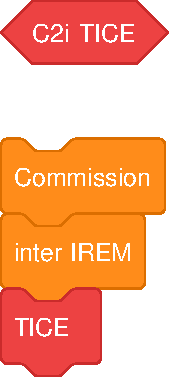
\includegraphics[scale=1.5]{logo_c2it_scratch}\\[2cm]
    Création de blocs avec Scratchblocks}
\author{%
    Commission inter IREM\footnote{Institut de Recherche sur l'Enseignement des Mathématiques} TICE\\
    
\includegraphics[height=1cm]{fig-c2it}
    }
\date{\today}




\begin{document}



%   Titre
\maketitle
\thispagestyle{empty}

%   Sommaire
\newpage
\tableofcontents


\newpage

\section{Scratchblocks}


L’extension \textbf{scratchblocks4} (aussi appelée \textit{Block Plugin}) est un outil permettant de construire et de générer des images de blocs à partir de lignes de code.
\\ 
Utile à toutes celles et ceux qui souhaitent intégrer des images de blocs Scratch dans leurs documents, cet outil en ligne a été développé à l’origine pour le site de Scratch (wiki et forum).


Scratchblocks est disponible à partir de l'adresse \url{https://scratchblocks.github.io/}.

Voici un exemple de blocs générés directement à partir du site internet.

~\\

\begin{figure}[h]
    \centering
    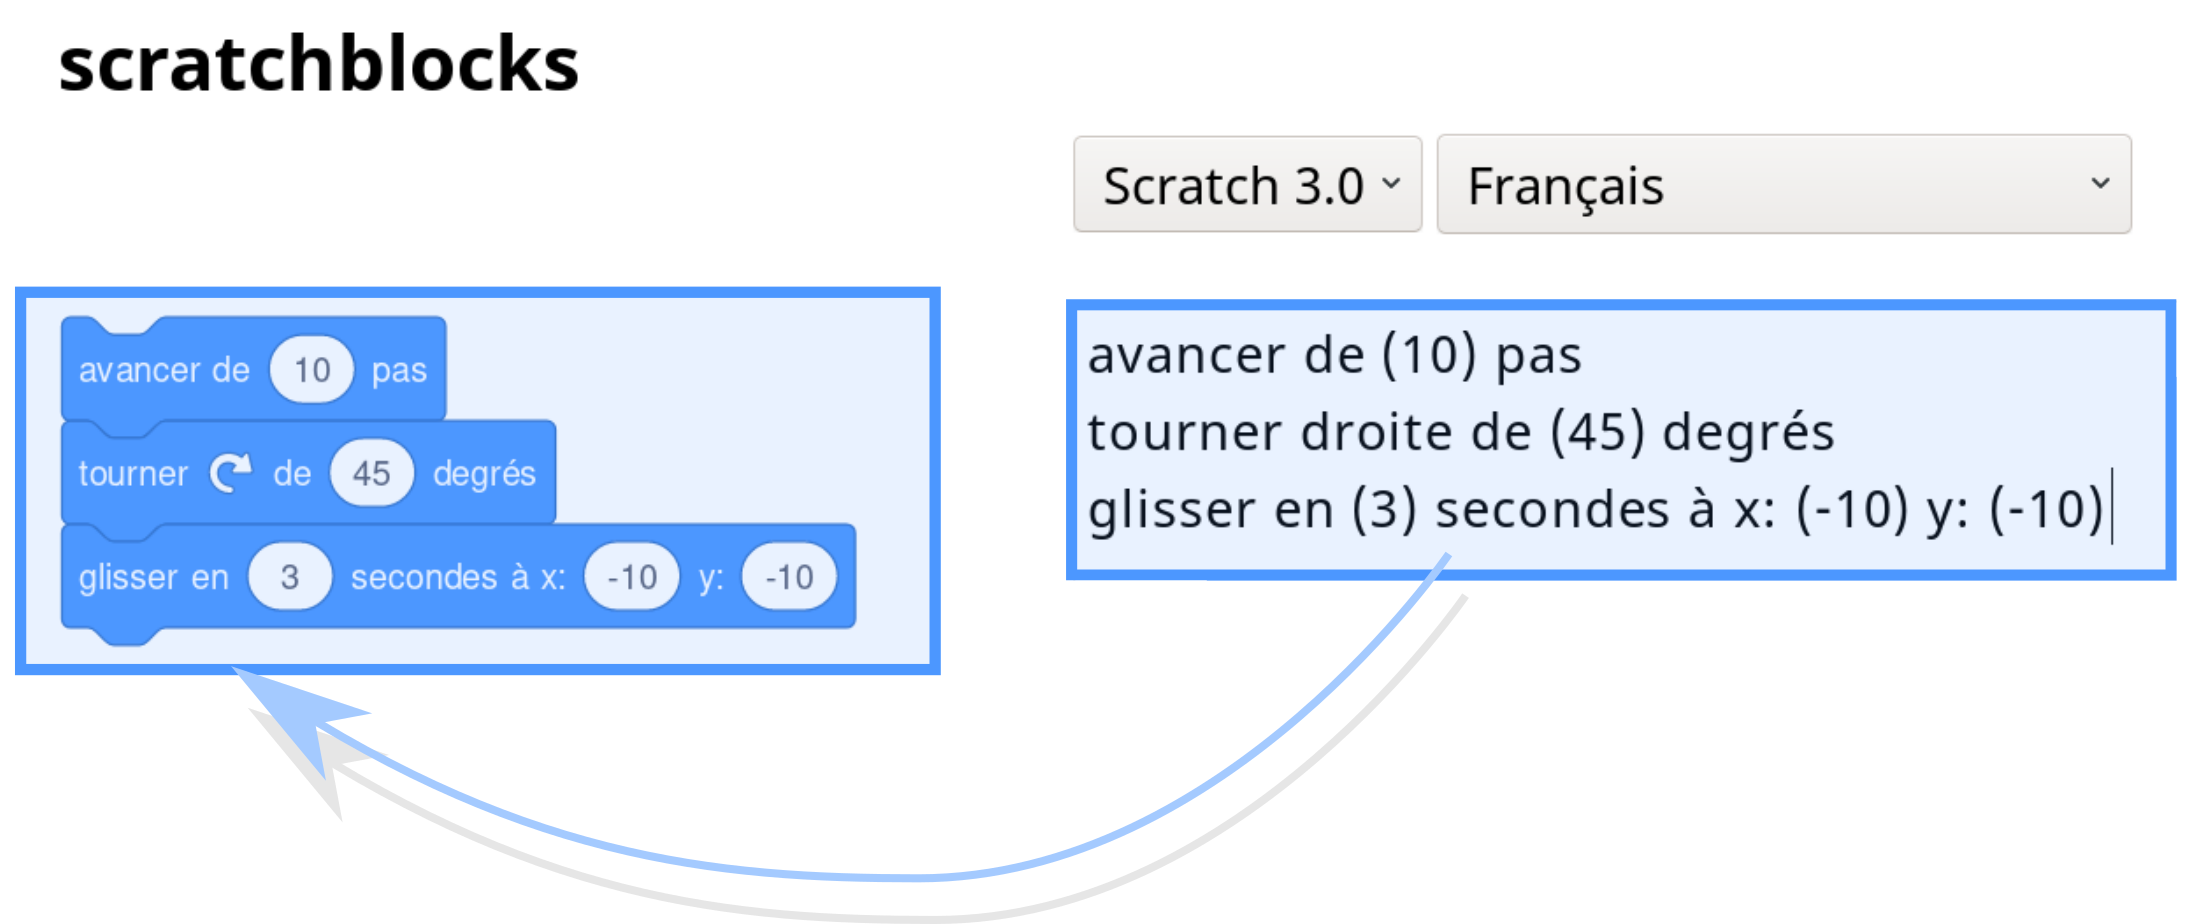
\includegraphics[width = 15cm]{res/app.png}
    \caption{Exemple de création de bloc à partir de quelques lignes de code}
    \label{}
\end{figure}

~\\

Dans cette publication, nous avons regroupé l'ensemble des commandes Scratch 3 reconnues par cet outil en ligne.

~\\

\begin{figure}[h]
    \begin{minipage}[t]{0.45\linewidth}
        \centering
        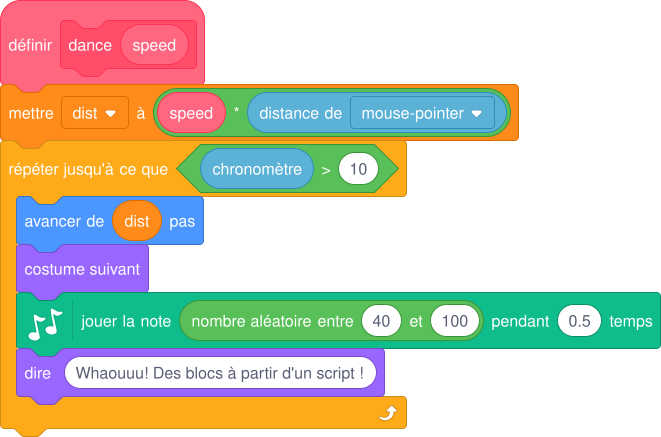
\includegraphics[width=\linewidth]{res/01_exemple.png}
        \caption{Des blocs "officiels"}
        \label{}
    \end{minipage}
    \hfill
    \begin{minipage}[t]{0.45\linewidth}
        \centering
        
\includegraphics[width=2cm]{res/fig-c2i-scratch}
        \caption{Des blocs "personnalisés"}
        \label{}
    \end{minipage}
\end{figure}


\newpage
\section{Blocs de base}

\pagestyle{scratch}




\subsection{Blocs Mouvement}

\vsScratch{2}{21}{1.82}{
	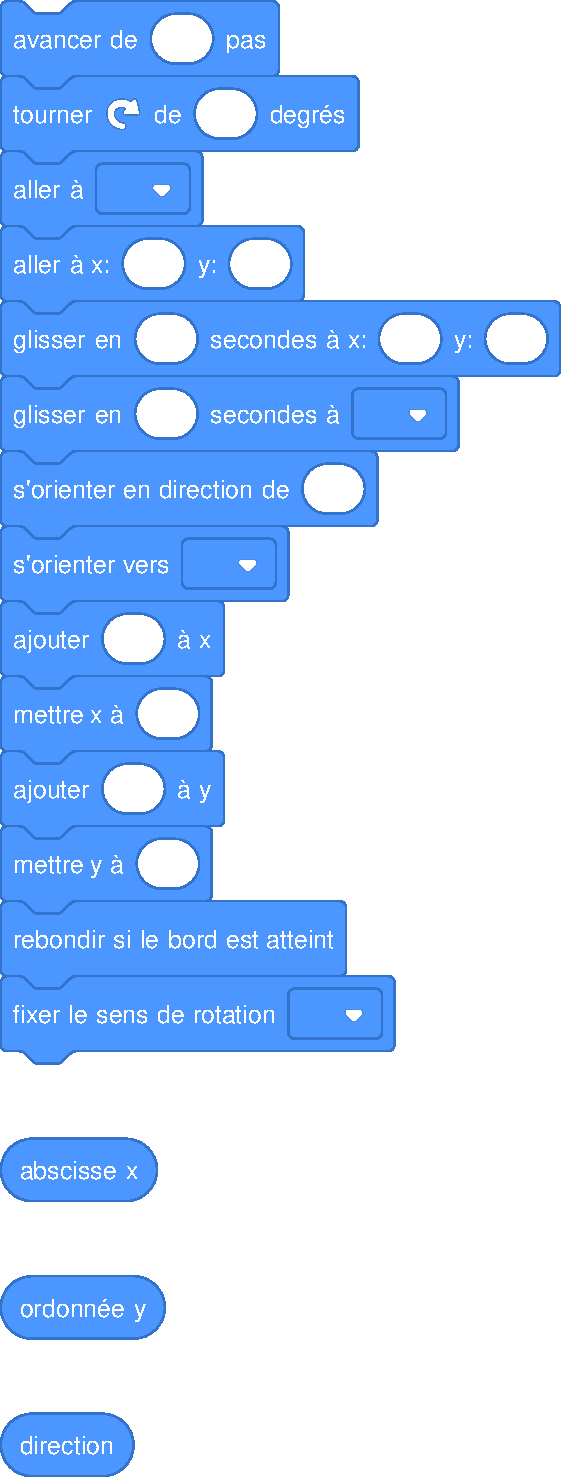
\includegraphics[scale=0.6]{./res/svg/scratchblocks_mouvement}
}



\subsection{Blocs Apparence}

\vsScratch{24}{42}{1.76}{
	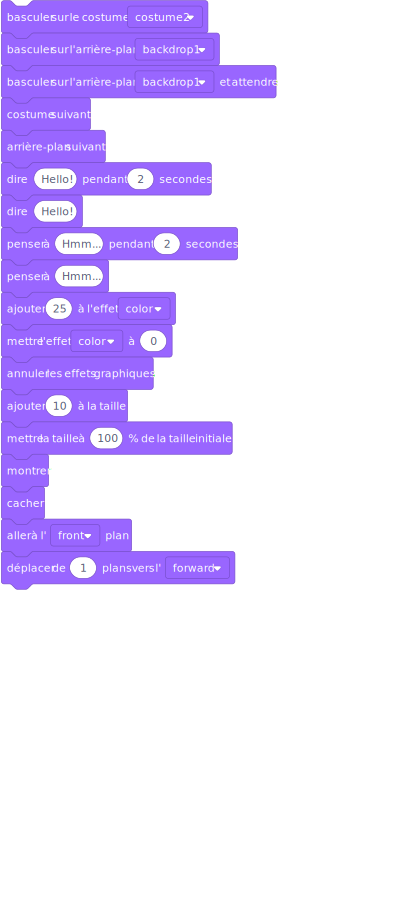
\includegraphics[scale=0.6]{./res/svg/scratchblocks_apparence}
}



\subsection{Blocs Son}

\vsScratch{45}{54}{1.89}{
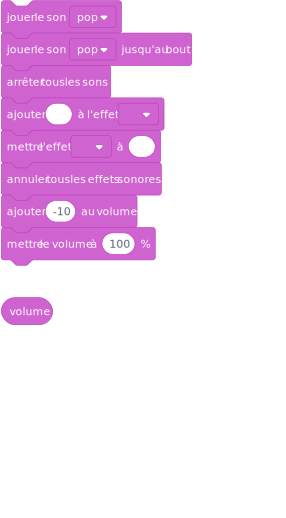
\includegraphics[scale=0.6]{./res/svg/scratchblocks_son}
}



\subsection{Blocs Évènements}

\vsScratch{57}{69}{2.28}{
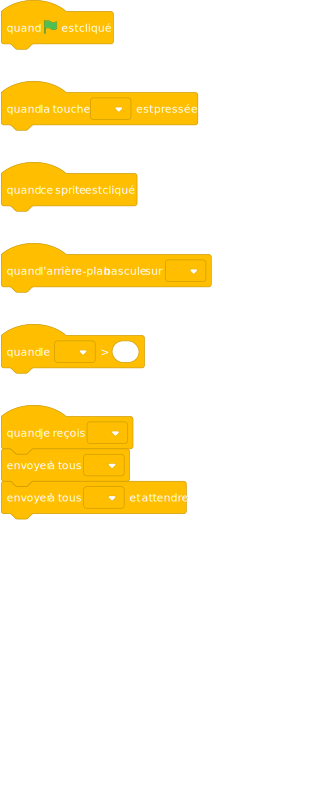
\includegraphics[scale=0.6]{./res/svg/scratchblocks_evenements}
}



\subsection{Blocs Contrôles}

\vsScratch{72}{88}{2.05}{
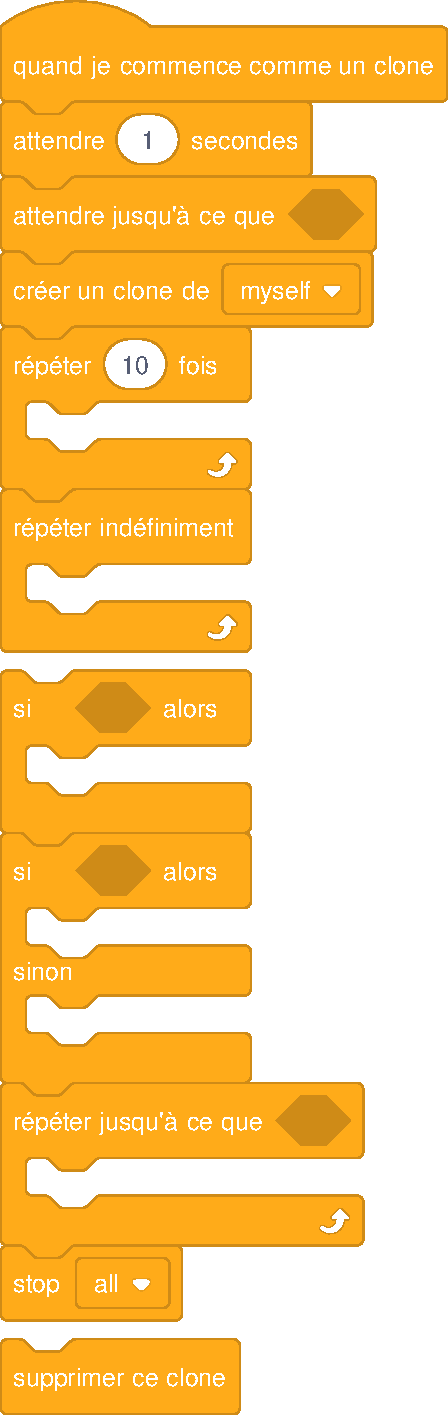
\includegraphics[scale=0.6]{./res/svg/scratchblocks_controle}
}



\subsection{Blocs Capteurs}

\vsScratch{91}{107}{3.05}{
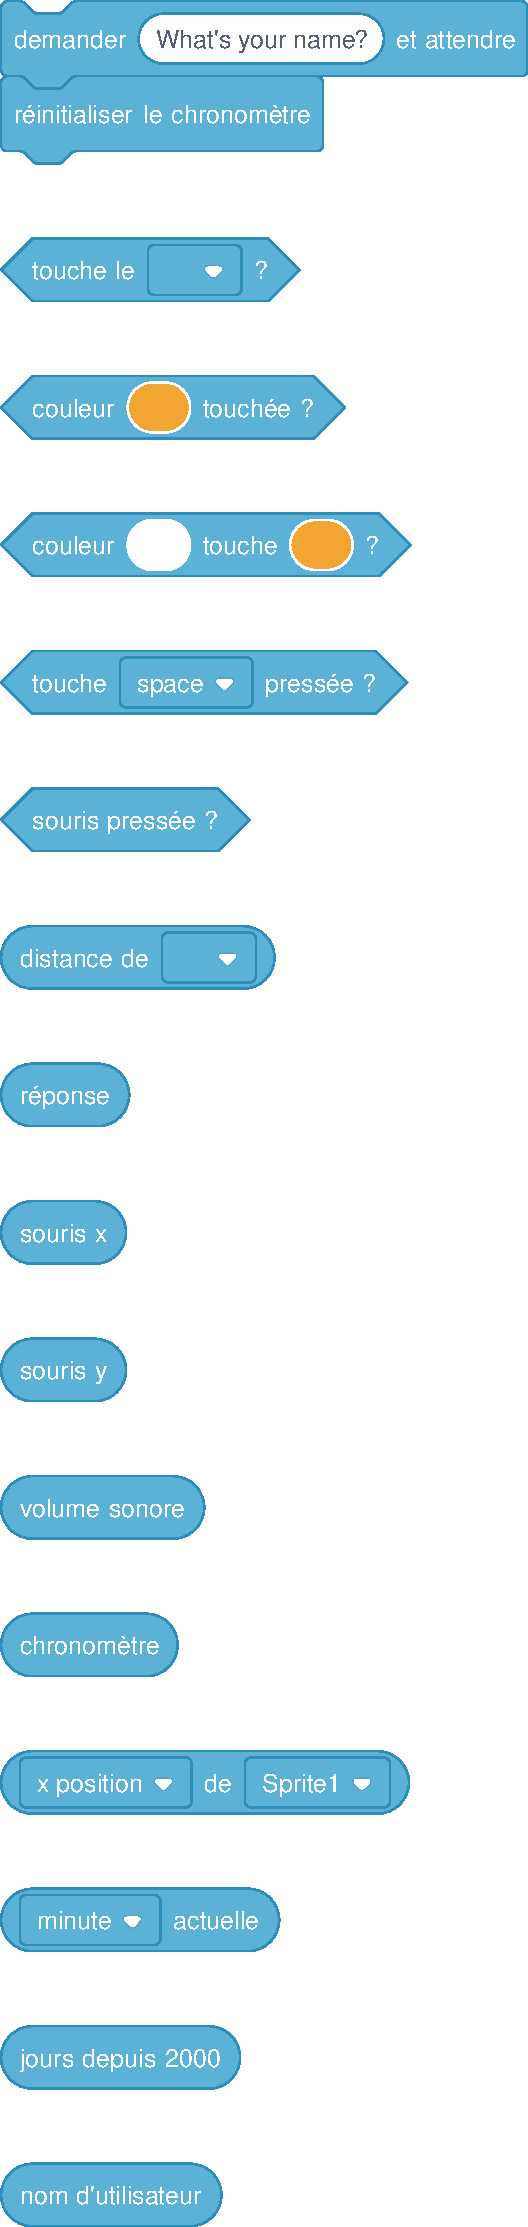
\includegraphics[scale=0.57]{./res/svg/scratchblocks_capteurs}
}



\subsection{Blocs Opérateurs}

\vsScratch{111}{128}{2.77}{
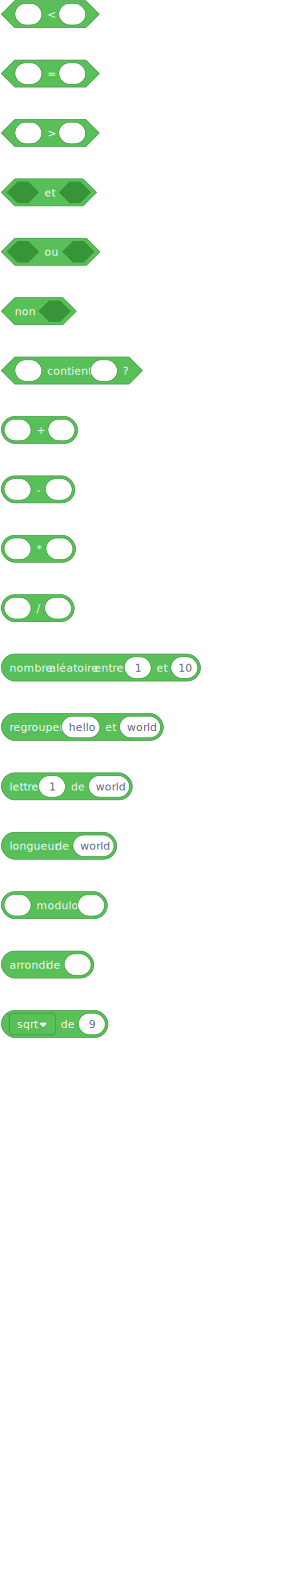
\includegraphics[scale=0.51]{./res/svg/scratchblocks_operateurs}
}



\subsection{Blocs Variables}

\vsScratch{131}{153}{1.86}{
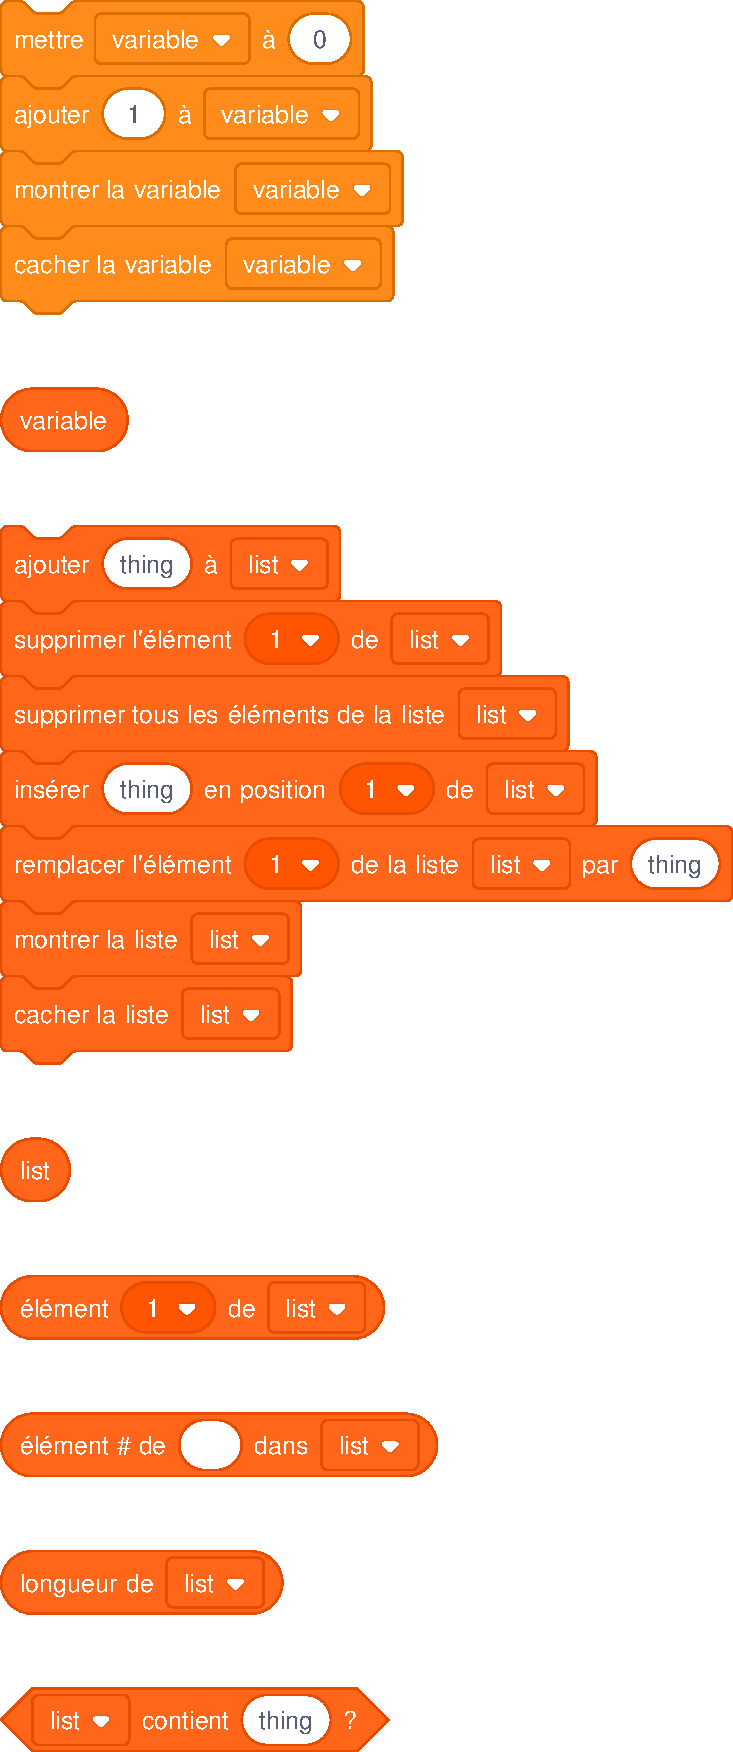
\includegraphics[scale=0.6]{./res/svg/scratchblocks_variables}
}



\subsection{Mes Blocs}

\vsScratch{156}{158}{1.95}{
\includegraphics[scale=0.6]{./res/svg/scratchblocks_mesblocs}
}



\section{Blocs d'extensions}

\subsection{Blocs Musique}

\vsScratch{160}{167}{2.15}{
	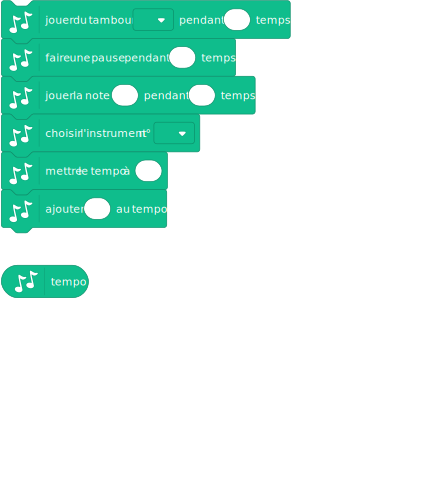
\includegraphics[scale=0.6]{./res/svg/scratchblocks_extension_musique}
}



\subsection{Blocs Stylo}

\vsScratch{170}{178}{2.22}{
	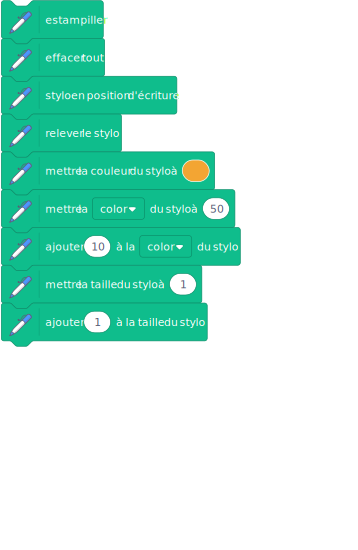
\includegraphics[scale=0.6]{./res/svg/scratchblocks_extension_stylo}
}



\subsection{Blocs Détection video}

\vsScratch{181}{186}{2.28}{
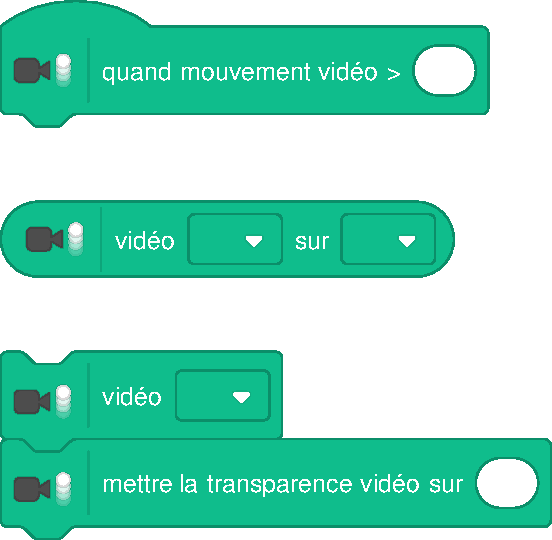
\includegraphics[scale=0.6]{./res/svg/scratchblocks_extension_detection_video}
}



\subsection{Blocs Synthèse Vocale}

\vsScratch{189}{191}{2.45}{
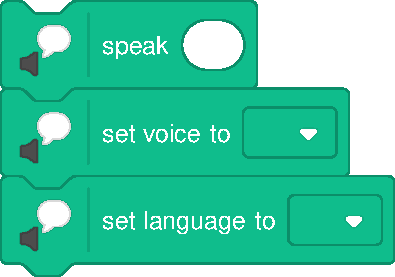
\includegraphics[scale=0.6]{./res/svg/scratchblocks_extension_synthese_vocale}
}



\subsection{Blocs Traduire}

\vsScratch{194}{196}{2.1}{
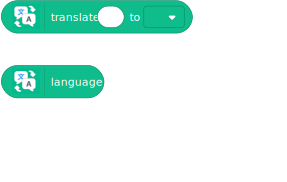
\includegraphics[scale=0.6]{./res/svg/scratchblocks_extension_traduction}
}



\subsection{Blocs Makey-Makey}

\vsScratch{198}{200}{2.05}{
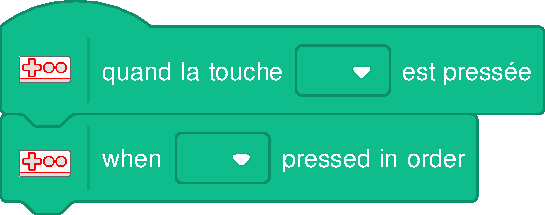
\includegraphics[scale=0.6]{./res/svg/scratchblocks_extension_makeymakey}
}



\subsection{Blocs \mb}

\vsScratch{202}{217}{2.18}{
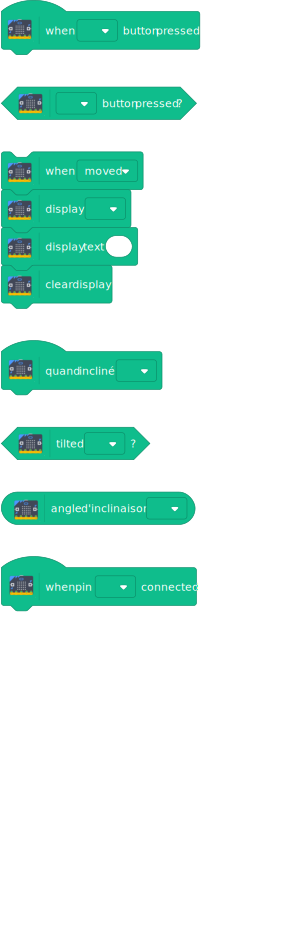
\includegraphics[scale=0.6]{./res/svg/scratchblocks_extension_microbit}
}



\subsection{Blocs LEGO Mindstorm}

\vsScratch{220}{240}{1.9}{
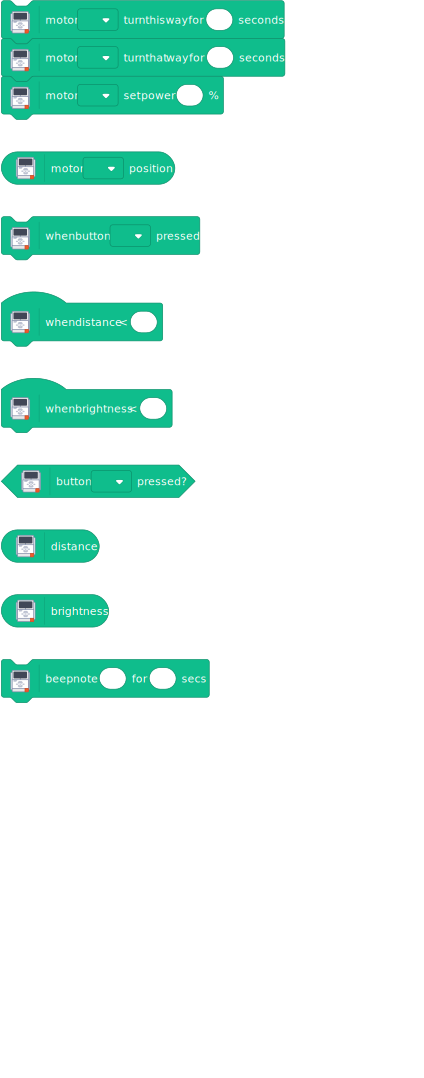
\includegraphics[scale=0.6]{./res/svg/scratchblocks_extension_LEGO_mindstorm}
}



\subsection{Blocs LEGO Wedo}

\vsScratch{242}{267}{1.38}{
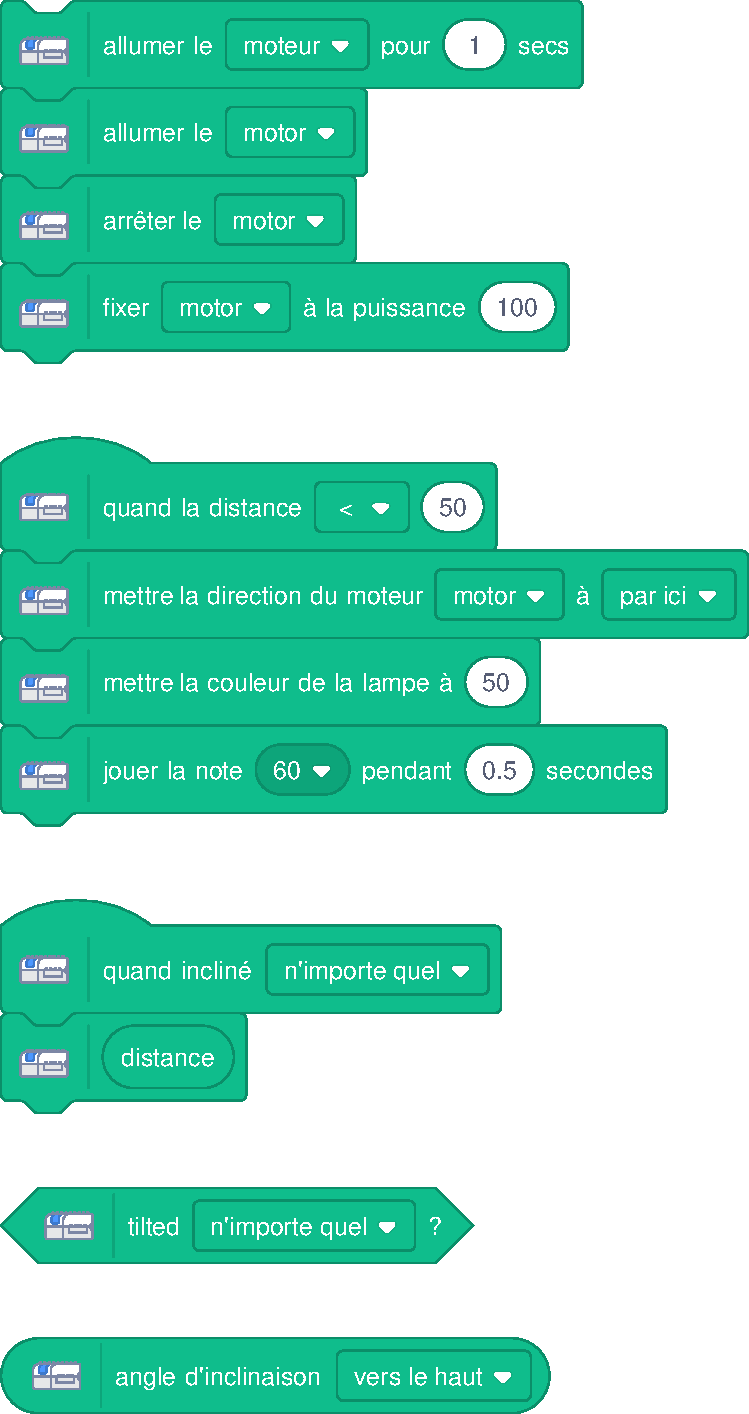
\includegraphics[scale=0.6]{./res/svg/scratchblocks_extension_LEGO_wedo}
}



%   A propos de la brochure
\newpage
\pagestyle{plain}

\section{À propos de cette publication}

\subsection{Qui sommes-nous?}

La Commission Inter-IREM TICE (C2i TICE) est intégrée aux \textbf{IREM}.

Le réseau des Instituts de Recherche sur l’Enseignement des Mathématiques (IREM) associe des enseignants du primaire, du secondaire et du supérieur, pour mener en commun des réflexions sur l’enseignement des mathématiques et proposer ensuite des formations, des textes ou des publications aux professeurs de cette discipline.

Les commissions Inter-IREM sont des groupes de travail constitués de membres de différents IREM. Certaines sont centrées sur un cycle d’études, telles la COPIRELEM et les commissions Collège ou Lycée, d’autres sur un thème, telles les commissions Épistémologie, TICE ou Statistiques et probabilités, d’autres sur un type d’activité, telle la commission Repères IREM ou Publimath.

La Commission Inter-IREM TICE (C2i TICE) s’intéresse à tous les aspects relatifs aux TICE (Technologie de l’Information et de la Communication pour l’Enseignement) dans l’enseignement des mathématiques.
Elle a pour objectifs de : faire le point sur les différentes utilisations des TICE ; collecter, orienter, structurer et harmoniser les travaux de recherche au sein des IREM ; ouvrir de nouveaux champs de recherche concernant l’utilisation de l’outil numérique ; préparer et intervenir à des colloques et universités d’été en collaboration avec les organismes institutionnels ; suivre les évolutions techniques et réfléchir à leur intérêt pour l’enseignement.

\begin{center}
    
\includegraphics[width=0.5\linewidth]{res/fig-c2it}
\end{center}


\subsection{Liens utiles}
\begin{description}
    \item[Les sites de la commission inter IREM TICE] et des IREM ~\\
        site de ressource de la commission : \url{http://tice.univ-irem.fr}\\
        page de la commission (site IREM) : \url{http://url.univ-irem.fr/c2itice}\\
        page d'accueil des IREM : \url{http://www.univ-irem.fr/}
    \item[Accès en ligne à Scratch] ~\\
        \url{https://scratch.mit.edu/projects/editor/}
    \item[Installation en local] Sous Windows ou MacOS\\
		\url{https://scratch.mit.edu/download}
	\item[Autre lien]  ~\\
 		\url{https://fr.scratch-wiki.info/wiki/Scratch_3.0#Refonte_des_blocs}
\end{description}




\end{document}